\chapter{Thảo luận\label{chapter:discussion}}

\section{Tóm tắt phát hiện}
Bảng~\ref{tab:findings} gom phát hiện chính cho mỗi câu hỏi nghiên cứu, cùng
độ mạnh bằng chứng hiện tại. Kết quả an toàn (RQ2) không phụ thuộc môi trường đo
chút nào. Kết quả di chuyển (RQ4) phụ thuộc theo một trục duy nhất, vì thời gian
build là phép đo thời gian, nên được báo dạng tỷ lệ ghép cặp. Kết quả hiệu năng và
tài nguyên phụ thuộc môi trường, và phép chia trung thực giờ nằm trong RQ1 chứ không
giữa các chương. Điểm gối bão hoà, so sánh quá tải, và
so sánh tài nguyên được giải quyết trên máy chủ Mục~\ref{sec:testbed}, và tái lập
qua kiểm soát bộ cấp phát. Đuôi xa dưới bão hoà vẫn chưa giải quyết, vì lý do
thuộc máy chứ không phải phân tích.

\begin{table}[tp]
\centering
\caption[Tóm tắt phát hiện theo câu hỏi nghiên cứu]{Tóm tắt phát hiện theo câu hỏi nghiên cứu và độ mạnh bằng chứng hiện tại.
\label{tab:findings}}
\renewcommand{\arraystretch}{1.25}
\begin{tabular}{@{}p{0.06\linewidth} p{0.62\linewidth} p{0.22\linewidth}@{}}
\hline\hline
RQ & Phát hiện chính & Trạng thái bằng chứng \\
\hline
RQ1 & Câu trả lời chia tại bão hoà. Dưới đó các biến thể đồng ý trong $\PFiftyRange\,\mu$s
($\PFiftySpread\%$) ở trung vị và không có thứ tự đuôi nào phân giải được. Số đầu-cuối chỉ
$\BudgetCoreShareMax\%$ thao tác, nên không thể giới hạn hiệu ứng ngôn ngữ trong mọi trường hợp, trong khi
thao tác đo riêng nhanh hơn $\BudgetCoreRatio\times$ ở \BudgetCoreFaster. Qua
bão hoà chúng phân kỳ dứt khoát: \OverloadSustainedFaster{} duy trì
$\OverloadThrRatio\times$ thông lượng của \OverloadSustainedSlower{} ở
$\OverloadLoad$~kops/s, trong \OverloadThrAgree{} lần lặp dưới cả hai bộ cấp phát. & Quá tải và
thao tác: đã giải quyết. Đuôi xa: chưa giải quyết trên máy này. Cơ chế: đã kiểm. Primitive riêng
không đủ \\
RQ2 & Cả bảy lớp an toàn bộ nhớ và tranh chấp dữ liệu tiêm được ngăn lúc biên dịch trong
Rust an toàn, trong khi ở C++ mỗi lớp biên dịch và chỉ bị bắt, nếu có, lúc runtime và không bộ dò lỗi đơn lẻ
nào. Bảo đảm dừng ở đó: bảy lớp biên biên dịch cả hai ngôn ngữ, và
trên rò rỉ và tràn bản build release công cụ C++ báo điều Rust không. &
Cuối cùng \\
RQ3 & Phạt bộ nhớ tái lập: thêm $\RssLangDiffLo$--$\RssLangDiffHi$~MiB peak RSS trong
bản build Rust dưới \emph{cả hai} bộ cấp phát, nhỏ hơn một bậc độ lớn so với
$\RssAllocDiffLo$--$\RssAllocDiffHi$~MiB của bộ cấp phát. CPU đảo giữa các chế độ: Rust tiêu tối đa
$\CpuDiffAbsMax$ điểm phần trăm ít hơn dưới bão hoà và $\OverloadCpuPerOpRatio\times$ nhiều hơn
mỗi thao tác hoàn thành phía trên. & Bộ nhớ: đã giải quyết, chưa giải thích. CPU: đã giải quyết cả hai
chế độ, dấu đối \\
RQ4 & Đường nối nhỏ và giữ lõi không \texttt{unsafe} lúc biên dịch. Đo so với
cùng thao tác gọi bản địa, không phát hiện chi phí và mọi thuế được giới hạn ở
$\FfiOpBoundPct\%$ một thao tác. Chi phí thật là thiết kế API. Lõi vẫn lộ lúc chạy
với lỗi bộ nhớ ở host C++ chia không gian địa chỉ. Trên các trục áp dụng ngoài
đường nối, $\BuildDepShareCpu\%$ build sạch Rust là mã bên thứ ba và mã riêng dự án biên dịch bằng $\BuildAllFirstPartyCpuRatio$ lần CPU \texttt{g++} cần, thứ tự
dấu chân đảo theo chính sách liên kết, và thành phần so sánh giải quyết $\DepsCore$ crate.
& Cuối cùng. Giây build tuyệt đối gắn host, tỷ lệ thì không \\
\hline
\end{tabular}
\end{table}

\section{Thảo luận về các câu hỏi nghiên cứu}\label{sec:rqdiscussion}
\paragraph{RQ1 (độ dự đoán được).} RQ1 có hai nửa, dưới bão hoà và qua nó, và
chiến dịch trả lời chúng đủ khác để báo cáo một mình sẽ bóp méo
kết quả.

Dưới bão hoà hai ngôn ngữ tương đương về hành vi trung tâm, với biên độ không triển khai
nào để ý. Khác biệt ghép cặp nhỏ ở trung vị vượt hiệu chỉnh là
một phần nhỏ của thao tác $80\,\mu$s. Đuôi xa trong chế độ này là chuyện khác, và triển khai
cũng quan tâm. Ở đó kết quả là null mà máy này không thể biến thành
thứ tự, nên tương đương tuyên bố ở đây không chạm tới nó. Kết quả trung tâm nhất quán với
bằng chứng rộng hơn rằng
kiểm tra an toàn của Rust phần lớn được CPU out-of-order hiện đại
hấp thụ~\cite{balasubramanian2017rust,emmerich2019drivers}. Nó cũng yếu hơn
trông, vì lý do Mục~\ref{sec:budget} nêu. Thao tác hai ngôn ngữ
thực thi là $\BudgetCoreShareMax\%$ những gì quét đo. Null đầu-cuối trong
thiết kế chi phối bởi đánh thức giữa luồng do đó nói về thiết kế chứ không
về ngôn ngữ. Đo riêng, thao tác khác $\BudgetCoreRatio\times$.

Qua bão hoà câu trả lời đổi loại, và đây là kết quả duy nhất trong nghiên cứu trả lời
RQ1 đúng theo nghĩa RQ1. Bản build C++ duy trì $\OverloadThrRatio$ lần thông lượng của
bản Rust trong khi tiêu nhiều CPU hơn mỗi thao tác hoàn thành, tái lập được và ở sàn
đã hiệu chỉnh của cả họ kiểm định (Mục~\ref{sec:overload}). Vậy dạng thực tế câu trả lời RQ1
không phải lựa chọn ngôn ngữ vô quan với độ dự đoán. Nó vô quan \emph{cho đến khi
dịch vụ không còn chịu tải}, và lúc đó nó quyết định bao nhiêu
công việc vẫn được làm. So sánh dừng ở tải danh nghĩa, như hầu hết trong tài liệu
này, sẽ kết luận ngược với cùng bộ máy.

Điều đó đặt lại công trình tiền nhiệm gần nhất thay vì chỉ đồng ý. Arvidsson và Kaller
đo đại lượng này cho thủ tục mặt điều khiển 5G và thấy phần trăm thứ 99 của Rust suy giảm
nhanh hơn qua ngưỡng tốc độ yêu cầu. Họ truy về
\texttt{async}/\texttt{await} không stack, cho phép chuyển ngữ cảnh ngay trước khi thao tác I/O
bắt đầu~\cite{arvidsson2025async}. Mục~\ref{sec:relatedwork} chấp nhận sự quy kết đó, và
nghiên cứu này được xây để loại nhiễu đằng sau: một worker mỗi shard qua hàng đợi chặn có giới hạn,
và không runtime bất đồng bộ hai bên.

Mục~\ref{sec:rqs}
cam kết trước mỗi kết quả sẽ có nghĩa gì, và nhánh thứ hai là nhánh
kích hoạt. Suy giảm qua ngưỡng tốc độ xuất hiện với mô hình đồng thời giữ cố định, nên
runtime bất đồng bộ không thể là nơi duy nhất hiệu ứng như vậy bắt đầu. Dự đoán cũng
đặt tên nơi nhìn trước nếu điều đó xảy ra: kiểm tra biên và tràn
~\cite{zhang2022runtime,harris2023morello}. Phần đó sai. Hiệu ứng
chỉ xuất hiện khi đường bàn giao tranh chấp, trỏ thay vào hai primitive chặn của
hai thư viện chuẩn ghi trong Bảng~\ref{tab:idioms}. Mục~\ref{sec:contention}
rồi kiểm tra liệu các primitive đó riêng giải thích khoảng cách, và chúng không tái tạo
thứ tự toàn dịch vụ ở mức ý nghĩa. Điều đó thu hẹp nguyên nhân vào công việc thêm trên đường bàn giao C++
chứ không phải mô hình an toàn. Ghi rằng dự đoán giải quyết ngược giả thuyết đầu
của chính nó, và microbenchmark theo sau tinh chỉnh quy kết thay vì xác nhận,
hữu ích hơn cho nghiên cứu sau hơn là lặng thay bằng lời giải thích còn sống.

\paragraph{RQ2 (an toàn).} Kết quả không phụ thuộc môi trường. Điều làm nó
thú vị không phải nửa xác nhận kỳ vọng, mà nửa giới hạn nó. Trong
phạm vi bảo đảm tuyệt đối theo một nghĩa cụ thể, và khác biệt với C++ là khác
loại chứ không phải mức độ. Trình biên dịch từ chối build loại trừ lỗi khỏi
mọi thực thi. Bộ dò lỗi chỉ loại trừ khỏi thực thi bài kiểm thử có công cụ
tình cờ đi qua. Điều tuyệt đối là độ phủ thực thi, không phải độ rộng danh mục.
Phạm vi vẫn là $\FaultClasses$ chương trình viết cho nó.
Điều đó khớp bằng chứng CVE rằng lỗi an toàn bộ nhớ Rust luôn liên quan
\texttt{unsafe}~\cite{xu2021rustcve}, và cảnh báo unsafety vẫn lan
qua phụ thuộc~\cite{evans2020rust}, đó là lý do giữ lõi không \texttt{unsafe}
quan trọng. Seam double-free là bằng chứng đó tái tạo trong điều kiện kiểm soát: lớp
duy nhất trong danh mục mà Rust an toàn từ chối và Rust unsafe không.

Ca duy nhất vượt chương trình đã viết là lỗi vòng đời của
Mục~\ref{sec:safetyresults}. Nó được tìm trong hiện thực, không viết cho
danh mục, và sửa bức tranh hai hướng. Nó củng cố lập luận
chi phí. Một lỗi thật trong mã viết để đúng sống sót toàn bộ bộ xác minh
của nghiên cứu này, tức kiểm thử, vector tương đương và ba bộ dò lỗi, chỉ vì
không gì đi qua đường đó. Phát hiện runtime phụ thuộc độ phủ kiểm thử là đề xuất
yếu hơn trong thực tế so với trong bảng mà mỗi hàng được lái có chủ đích.

Nó cũng
thu hẹp điều có thể ghi cho Rust, vì đóng góp ngôn ngữ ở đó là bounds
check chứ không phải chứng minh. Rust an toàn biến undefined behaviour thành panic xác định, đó là
tuyên bố khác và kém hơn ngăn lỗi. Tổng quát hoá trung thực là
bảo đảm đáng ngân sách là \emph{kiểm tra mặc định} chứ không phải \emph{loại trừ lúc
biên dịch}. Nguyên nhân gốc đáng đặt tên, vì đó là rủi ro của phương pháp
chứ không phải ngôn ngữ nào. Đặc tả nêu lệnh cấm mà không gán
cơ chế để mỗi hiện thực lỗi theo idiom riêng. Hai idiom ở đây là
panic và use-after-free.

Nơi bảo đảm dừng quan trọng không kém cho nhà cung cấp quyết định Rust mua gì, và hai
lớp biên minh hoạ vì lý do khác nhau. Deadlock thứ tự khóa cho thấy Rust
suy luận về \emph{aliasing} chứ không về \emph{thứ tự acquisition}. Guard \texttt{Mutex} là
giá trị thường mà borrow checker theo dõi vòng đời hoàn hảo, và theo dõi hoàn hảo
không nói hai luồng lấy khóa theo thứ tự tương thích. Công cụ quanh ngôn ngữ xác nhận đây là biên chứ không phải artefact ví dụ tiêm.
Phát hiện deadlock tĩnh cho Rust là bài toán nghiên cứu đang hoạt động
riêng~\cite{zhang2026deadlock}, và bộ kiểm tra mô hình cho mã kernel Rust được thúc đẩy
rõ ràng bởi quan sát ownership và borrowing để lại tranh chấp dữ liệu, deadlock và
livelock vẫn chạm tới~\cite{tang2025converos}.

Lost update sắc hơn nữa. Nó thoát
ThreadSanitizer đúng lý do thoát borrow checker, như
Mục~\ref{sec:safetyresults} nêu. Với mọi truy cập đồng bộ đúng không có
truy cập không đồng bộ để tìm. Cũng không lớp lề. Trong nghiên cứu thực địa $105$
lỗi đồng thời thật, khoảng một phần ba ca không deadlock vi phạm thứ tự lập trình viên
định, không phải khóa của họ, và tác giả ghi ý định như vậy không diễn đạt
dễ qua khóa~\cite{lu2008mistakes}. Phân biệt
nó bộc lộ, giữa race dữ liệu và điều kiện đua, là điều cụm ``an toàn luồng'' thường gộp, và Rust chỉ loại bỏ
cái đầu.

Hệ quả thực hành là áp dụng Rust loại bỏ hoàn toàn một loại lỗi đồng thời
trong khi để nguyên loại kia. Loại còn lại là loại thất bại
im lặng, làm hỏng bộ đếm hay quyết định trạng thái thay vì crash. Kế hoạch di chuyển
coi ``an toàn bộ nhớ'' là ``an toàn đồng thời'' sẽ do đó lập ngân sách review và kiểm thử
sai. Đó là lý do biên được báo cáo như kết quả hạng nhất chứ không phải điều kiện.
Hình~\ref{fig:boundary} vẽ chính biên, với hai nửa
bảo đảm hai bên đường và cơ chế thực thi, hoặc vắng mặt
của nó, được đặt tên mỗi panel. Nó mang hai ca đồng thời thay vì cả bảy ngoài
bảo đảm, vì chúng là cặp làm rõ phân biệt, và
Bảng~\ref{tab:taxonomy} giữ toàn danh mục.

\begin{figure}[ht]
\centering
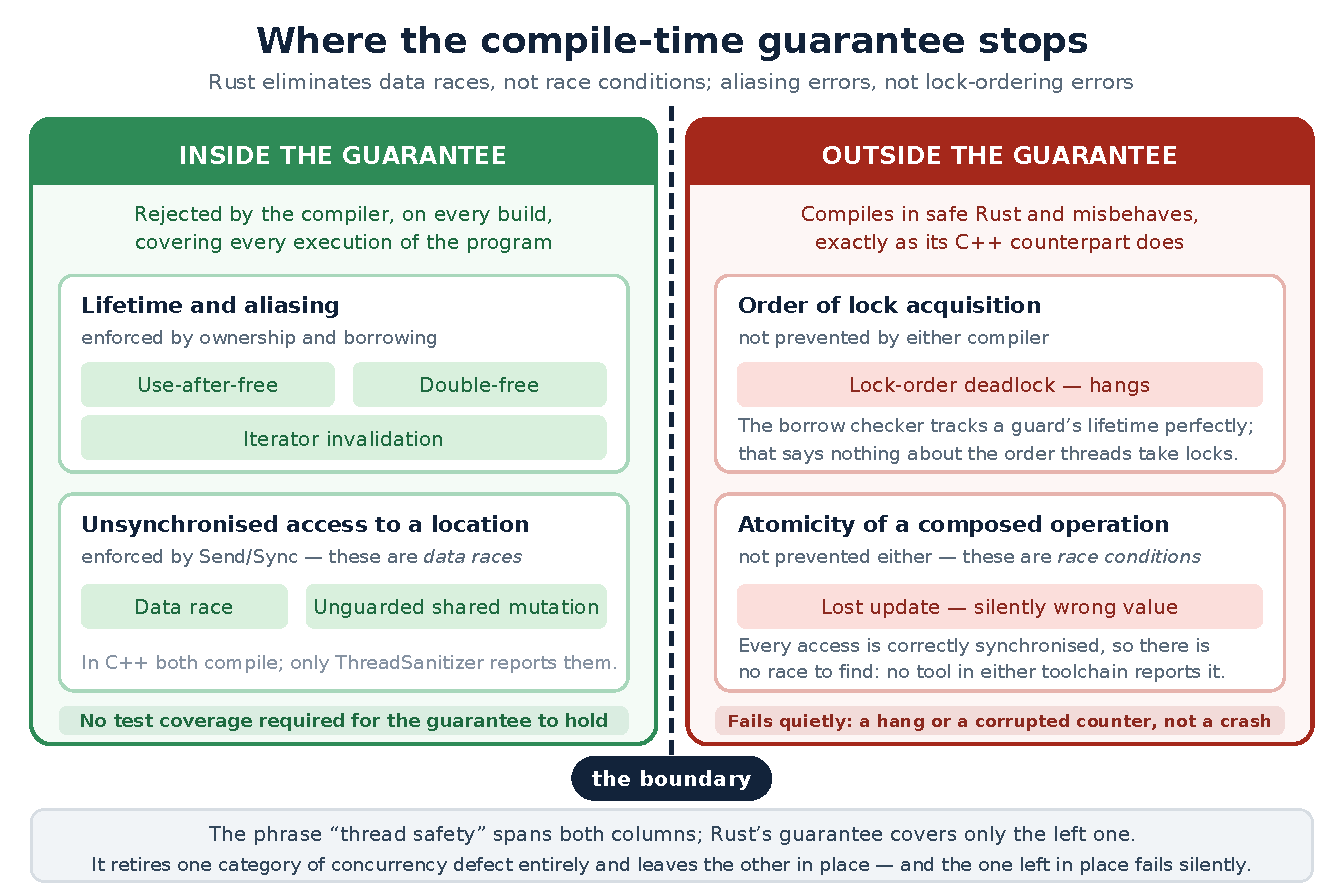
\includegraphics[width=0.78\linewidth]{diagrams/pdf/17_guarantee_boundary.pdf}
\caption[Nơi bảo đảm biên dịch của Rust dừng]{Nơi bảo đảm biên dịch dừng. Bên trái là các lớp Rust an toàn từ chối
hẳn, nhóm theo \emph{cơ chế} từ chối thay vì theo họ
lỗi: ownership và borrowing cho lỗi vòng đời và aliasing,
đó là lý do vô hiệu hoá iterator nằm cùng chúng, và kỷ luật \texttt{Send}/\texttt{Sync}
cho truy cập không đồng bộ vào một vị trí. Bên phải là các lớp danh mục đưa vào để tìm cạnh, mà không trình biên dịch nào ngăn. Sơ đồ đặt tên một
lớp mỗi cơ chế và không phải danh mục, mà
Bảng~\ref{tab:defectmap} liệt kê đầy đủ: use-after-move thuộc
các ca ownership bên trái và handle không an toàn luồng chia sẻ với \texttt{Send}/\texttt{Sync}
bên đó, trong khi rò rỉ, tràn bản build release, lỗi worker, seam double-free
và forgotten guard nằm cạnh hai ca bên phải. Cụm ``an toàn luồng'' trải
cả hai bên đường, và bảo đảm chỉ bao trái. Đường lại di chuyển thêm một lần
nữa so với sơ đồ thể hiện, vì chương trình viết \texttt{unsafe} vượt qua nó
tự nguyện.\label{fig:boundary}}
\end{figure}

